\bookchapter{Глава 42: Панорама больших моделей и практика работы с API}

\chapterintro{В предыдущих главах говорилось о том, «как сотрудничать с AI». Эта глава отвечает на более базовый вопрос: «Каким AI пользоваться? Как именно?» К августу 2026 года ландшафт больших моделей стал чрезвычайно богатым: на международной арене соперничают три лидера — GPT, Claude и Gemini, а в Китае пышным цветом расцвели DeepSeek, Tongyi Qianwen, GLM, Kimi и Doubao. У каждой модели свой характер и свои сильные стороны: удачный выбор удваивает результат при тех же усилиях, неудачный — наоборот. В этой главе вы не только познакомитесь с этими моделями, но и научитесь подключать их к своим приложениям через API, а также подбирать подходящий пакет лимитов (Token Plan) под свои задачи.}

\booksection{Ведущие международные модели: расстановка трёх лидеров}

К августу 2026 года на международном рынке больших моделей сложился «триумвират»: OpenAI (серия GPT), Anthropic (серия Claude) и Google (серия Gemini). У каждой компании яркий собственный почерк — познакомимся с ними по очереди.

\booksubsection{Серия OpenAI GPT-5.6: универсальный «шестигранный боец»}

OpenAI стояла у истоков волны больших моделей, и серия GPT до сих пор остаётся самой востребованной в мире. Вышедшая в июле 2026 года серия GPT-5.6 использует стратегию трёх уровней: флагман GPT-5.6 Sol рассчитан на задачи с требовательными рассуждениями, сбалансированный GPT-5.6 Terra — на повседневную разработку, а лёгкий GPT-5.6 Luna — на сценарии с высокой нагрузкой и низкой стоимостью. У всех трёх моделей контекстное окно в 1,05 млн токенов; все они поддерживают ввод изображений, вызов функций и структурированный вывод.

\begin{center}
\begin{tabularx}{\linewidth}{|X|X|X|X|X|}
\hline
\textbf{Модель} & \textbf{Позиционирование} & \textbf{Ввод (за 1 млн токенов)} & \textbf{Вывод (за 1 млн токенов)} & \textbf{Контекстное окно} \tabularnewline
\hline
GPT-5.6 Sol & Флагманские рассуждения & 5,00 долл. (около 36 юаней) & 30,00 долл. (около 217 юаней) & 1,05 млн токенов \tabularnewline
GPT-5.6 Terra & Сбалансированные повседневные задачи & 2,50 долл. (около 18 юаней) & 15,00 долл. (около 109 юаней) & 1,05 млн токенов \tabularnewline
GPT-5.6 Luna & Лёгкий, дешёвый & 1,00 долл. (около 7 юаней) & 6,00 долл. (около 44 юаней) & 1,05 млн токенов \tabularnewline
\hline
\end{tabularx}
\end{center}

\begin{center}\small\color{gray}Цены серии OpenAI GPT-5.6 (август 2026 г.)\end{center}

Ключевое преимущество серии GPT — сбалансированность: рассуждения, программирование, письмо, мультимодальность — без заметных слабых мест. Добавьте огромную экосистему плагинов и сообщество разработчиков OpenAI — самая проработанная документация и цепочки инструментов. Когда вы «не знаете, что выбрать», GPT — ответ по умолчанию, «который не подведёт даже с закрытыми глазами». Но есть минусы: доступ из Китая требует особых сетевых средств, по-китайски модель иногда звучит с «переводным акцентом», а цены API — выше среднего.

\textbf{Хорошая новость}\par

В августе 2026 года OpenAI объявила, что моделью по умолчанию для бесплатных пользователей стала GPT-5.6 Luna, а текстовый чат открыт без лимитов. Это значит, что базовые возможности GPT вы можете опробовать бесплатно — платить придётся только если нужны более мощные рассуждения или вызовы API.

\booksubsection{Серия Anthropic Claude: эталон программирования и строгости}

Если GPT — универсальный игрок, то Claude — «потолок» в программировании. Серия Claude от Anthropic долго время с большим отрывом лидирует в SWE-bench (бенчмарке программной инженерии); качество генерации кода и способность доводить проекты до промышленного уровня — первые в отрасли. Что ещё ценнее, у Claude самый низкий в сети уровень галлюцинаций (вероятности выдачи ложной информации) — всего около 1\%. Поэтому он особенно подходит для высокоточных сценариев: наука, юриспруденция и т. п.

Ещё один козырь Claude — сверхдлинный контекст: контекстное окно в 1 млн токенов позволяет за один раз «прочитать» контракт на сотни страниц или целую кодовую базу, ничего не упустив. В задачах вроде рефакторинга кода и анализа длинных документов он практически незаменим. Claude Code как инструмент AI-программирования в терминале к середине 2026 года достиг годовой выручки в 2,5 млрд долларов — лучшее подтверждение признания способностей Claude к программированию.

\begin{center}
\begin{tabularx}{\linewidth}{|X|X|X|X|X|}
\hline
\textbf{Модель} & \textbf{Позиционирование} & \textbf{Ввод (за 1 млн токенов)} & \textbf{Вывод (за 1 млн токенов)} & \textbf{Контекстное окно} \tabularnewline
\hline
Claude Fable 5 & Флагман & 10,00 долл. (около 72 юаней) & 50,00 долл. (около 362 юаней) & 1 млн токенов \tabularnewline
Claude Opus 4.8 & Профессиональный & 5,00 долл. (около 36 юаней) & 25,00 долл. (около 181 юаня) & 1 млн токенов \tabularnewline
Claude Sonnet 5 & Оптимум по цене и качеству & 2,00 долл. (около 14 юаней) & 10,00 долл. (около 72 юаней) & 1 млн токенов \tabularnewline
\hline
\end{tabularx}
\end{center}

\begin{center}\small\color{gray}Цены серии Anthropic Claude (август 2026 г.; Sonnet 5 — по льготной цене)\end{center}

Слабое место Claude — цена: у Fable 5 самая высокая цена вывода среди всех моделей — 50 долларов за миллион токенов. Мультимодальные возможности (понимание изображений и видео) тоже сравнительно слабее. Для индивидуальных разработчиков с ограниченным бюджетом Sonnet 5 в льготный период даёт особенно выгодное соотношение цены и качества.

\booksubsection{Серия Google Gemini: король мультимодальности}

Серия Gemini от Google к 2026 году доросла до версии 3.1 Pro. Главный козырь Gemini — нативная мультимодальность: точный разбор текста и изображений, безошибочное распознавание таблиц через OCR, эффективное извлечение кадров видео, плюс глубокий разбор аудио и видео. Модель глубоко интегрирована с экосистемой Google (поиск, почта, облачные сервисы) и блестяще справляется с поиском информации в реальном времени и межмодальным пониманием. Gemini также поддерживает сверхдлинный контекст ввода в 2 млн токенов — это самое большое контекстное окно среди существующих моделей.

Gemini позиционируется как «выбор номер один для научных рассуждений и мультимодальных задач». Если ваш проект связан с анализом большого числа изображений, пониманием видео или научными вычислениями, у Gemini почти нет конкурентов. Но в генерации кода по чистому тексту он немного уступает Claude, а по-китайски выражается менее естественно, чем китайские модели.

\begin{center}
\begin{tabularx}{\linewidth}{|X|X|X|X|}
\hline
\textbf{Параметр сравнения} & \textbf{GPT-5.6} & \textbf{Claude Fable 5} & \textbf{Gemini 3.1 Pro} \tabularnewline
\hline
Общий балл & 94.8 & 95.0 & 92.1 \tabularnewline
Навыки программирования (SWE-bench) & 74.9\% & 64.3\% (Pro) & Средний \tabularnewline
Контекстное окно & 1,05 млн токенов & 1 млн токенов & 2 млн токенов \tabularnewline
Мультимодальность & Сбалансированная & Слабая & Самая сильная \tabularnewline
Уровень галлюцинаций & Низкий & Самый низкий (около 1\%) & Низкий \tabularnewline
Доступность в Китае & Требует особой сети & Требует особой сети & Требует особой сети \tabularnewline
API-экосистема & Самая развитая & В развитии & Привязка к экосистеме Google \tabularnewline
\hline
\end{tabularx}
\end{center}

\begin{center}\small\color{gray}Сравнение трёх международных моделей (август 2026 г.)\end{center}

\begin{tcbwarn}{Внимание: реальные барьеры при использовании в Китае}
Для китайских разработчиков главное препятствие для GPT, Claude и Gemini — сетевой доступ. Пользоваться ими можно опосредованно — через прокси Azure, платформы-агрегаторы API и т. п., — но стабильность и легальность нужно оценивать самостоятельно. Если ваш проект предъявляет строгие требования к безопасности данных, лучше в первую очередь рассмотреть китайские модели.

\end{tcbwarn}

\booksection{Ведущие китайские модели: богатое разнообразие}

В 2026 году китайские большие модели перестали быть «догоняющими» и бегут наравне с лидерами, а в некоторых областях даже вырвались вперёд. В отличие от споров 2023 года о «моделях-обёртках», китайские флагманы 2026 года уже на равных с передовыми международными моделями в логических рассуждениях, генерации кода и понимании китайского языка — разрыв сократился до 5\% и меньше. Что ещё важнее, у китайских моделей есть незаменимые преимущества в китайскоязычных сценариях, стоимости и развёртывании с соблюдением норм.

\booksubsection{DeepSeek V4: король цены и качества}

DeepSeek — феномен среди китайских больших моделей. В начале 2025 года DeepSeek-V3 потряс рынок позицией «в десять раз дешевле GPT при равных возможностях» и получил в отрасли имя «линия уничтожения универсальных AI-моделей»: те, что дешевле, не так удобны, а те, что дороже, не дают такого объёма и щедрости. К августу 2026 года вышел официальный релиз DeepSeek V4-Pro: MoE-архитектура на 1,6 трлн параметров с активацией около 49 млрд, поддержка контекста в 1 млн токенов без потерь; соотношение цены и качества в коде считается общемировым потолком.

В DeepSeek V4 резко выросли агентные способности: бенчмарк DeepSWE подскочил с 12,8 до 62,7 (+390\%), а NL2Repo — с 38,5 до 61,5. API получил поддержку сразу двух протоколов — Responses API и Anthropic API — и уже совместим с популярными инструментами программирования вроде Codex и Claude Code. Это значит, что вы можете использовать API DeepSeek вместо API Claude прямо в Claude Code: затраты падают в несколько раз, а впечатления почти идентичны.

\begin{center}
\begin{tabularx}{\linewidth}{|X|X|X|X|X|}
\hline
\textbf{Модель} & \textbf{Позиционирование} & \textbf{Ввод (за 1 млн токенов)} & \textbf{Вывод (за 1 млн токенов)} & \textbf{Контекстное окно} \tabularnewline
\hline
DeepSeek V4 Pro & Флагманские рассуждения & 3 юаня (около 0,43 долл.) & 6 юаней (около 0,87 долл.) & 1 млн токенов \tabularnewline
DeepSeek V4 Flash & Лёгкий и быстрый & 1 юань (около 0,14 долл.) & 2 юаня (около 0,28 долл.) & 1 млн токенов \tabularnewline
\hline
\end{tabularx}
\end{center}

\begin{center}\small\color{gray}Цены серии DeepSeek V4 (август 2026 г., акционные)\end{center}

Сравнение цен: за 1 млн токенов ввода плюс 1 млн токенов вывода DeepSeek V4 Flash стоит около 0,42 доллара, GPT-5.6 Sol — около 35 долларов, а Claude Fable 5 — около 60 долларов. Разница достигает 80–140 раз.

\textbf{Осторожно: DeepSeek готовится поднять цены}\par

Официально DeepSeek 6 августа 2026 года объявил о «плане в ближайшее время заметно поднять цены на API» — акционные цены могут долго не продержаться. По слухам в СМИ, подорожание может достигнуть 30 раз; по состоянию на 14 августа окончательная схема цен не опубликована. Кроме того, официальный релиз DeepSeek V4 ввёл тарифы «пик–непик»: в часы пик вызовы стоят вдвое дороже. Следите за официальными объявлениями, чтобы знать актуальные цены.

\booksubsection{Tongyi Qianwen Qwen3.7 Max: корпоративный выбор Alibaba Cloud}

Серия Tongyi Qianwen (Qwen) от Alibaba Cloud, опираясь на экосистему Alibaba Cloud, имеет естественные преимущества в корпоративном развёртывании. Флагман июля 2026 года — Qwen3.7 Max: плотная модель на 235 млрд параметров с нативным контекстом 256K, расширяемым до 1 млн. Ключевые преимущества Qwen: зрелая open-source-экосистема (открыта вся линейка от 7B до 235B), точное понимание китайскоязычных сценариев и глубокая интеграция с инфраструктурой Alibaba Cloud.

\begin{center}
\begin{tabularx}{\linewidth}{|X|X|X|}
\hline
\textbf{Модель} & \textbf{Цена вывода (за 1 млн токенов)} & \textbf{Сценарии применения} \tabularnewline
\hline
qwen-turbo & 0,6 юаня & Простые вопросы-ответы, классификация текста, высокая нагрузка \tabularnewline
qwen-long & 2,0 юаня & Обработка сверхдлинного контекста (10 млн) \tabularnewline
qwen3.7-flash & 7,2 юаня & Обычные диалоги, генерация контента \tabularnewline
qwen3.7-plus & 12,0 юаня & Мультимодальность (изображения и видео), тексты на китайском \tabularnewline
qwen3.7-max & 36,0 юаней & Флагманские возможности для китайского языка, сложные задачи \tabularnewline
\hline
\end{tabularx}
\end{center}

\begin{center}\small\color{gray}Ступенчатые цены серии Tongyi Qianwen Qwen (август 2026 г.)\end{center}

Цены Qwen выстроены ступенями — от сверхдешёвого qwen-turbo (вывод 0,6 юаня за миллион токенов) до флагмана qwen3.7-max (вывод 36 юаней за миллион токенов), покрывая все сценарии — от простых вопросов-ответов до сложных рассуждений. Для компаний, уже работающих с Alibaba Cloud, Qwen — самый удобный вариант интеграции.

\booksubsection{Zhipu GLM-5.1: первое место среди китайских моделей в SWE-bench}

Серия GLM от Zhipu AI в 2026 году выглядела блестяще. GLM-5.1 занял первое место среди китайских моделей в SWE-bench: гибридная MoE-архитектура на 744 млрд параметров, поддержка контекста в 1 млн токенов. Его отличают точное понимание китайской семантики и поддержка легального частного развёртывания в Китае — это очень важно для финансов и госсектора, где требования к безопасности данных высоки. Цены GLM-5.1: ввод 6 юаней, вывод 24 юаня за миллион токенов — середина среди китайских моделей.

\booksubsection{Kimi K3: король сверхдлинных текстов}

Серия Kimi от компании Moonshot AI славится обработкой сверхдлинных текстов. Вышедший в июле 2026 года Kimi K3 имеет 2,8 трлн параметров и в ряде оценок сложных задач входит в мировой первый эшелон. Главные сценарии Kimi — анализ длинных кодовых баз и расширенный поиск по длинным документам: он может обработать текст целой книги или код целого проекта и блестяще справляется с задачами поиска «иголки в стоге сена». Цены у Kimi сравнительно высокие (вывод около 12–20 юаней за миллион токенов), но по цене и качеству в сценариях с длинными текстами ему нет равных.

\booksubsection{Doubao: универсальный игрок ByteDance}

Серия Doubao от ByteDance в 2026 году показывает стабильные результаты. Doubao Seed 2.1 Pro — флагманская модель Volcano Engine с контекстом 256K: в реальных тестах она работает стабильно, а в китайскоязычных сценариях особенно приятна. Преимущества Doubao: большие бесплатные пакеты токенов сразу после регистрации, хорошо проработанная интеграция с экосистемой Volcano Engine и одни из самых низких цен в Китае. Для новичков, которые хотят быстро попробовать AI-программирование, Doubao — вход без порога.

\begin{center}
\begin{tabularx}{\linewidth}{|X|X|X|X|X|X|}
\hline
\textbf{Параметр сравнения} & \textbf{DeepSeek V4} & \textbf{Qwen3.7 Max} & \textbf{GLM-5.1} & \textbf{Kimi K3} & \textbf{Doubao 2.1 Pro} \tabularnewline
\hline
Общий балл & 87.5 & 89.7 & 90.5 & 88+ & 85+ \tabularnewline
Навыки программирования & Очень сильные & Сильная & №1 в SWE среди китайских моделей & Сильная & Выше среднего \tabularnewline
Понимание китайского языка & Отлично & Отлично & Точно & Отлично & Отлично \tabularnewline
Контекстное окно & 1 млн & 256K-1M & 1 млн & Сверхдлинное & 256K \tabularnewline
Цена вывода (юаней за 1 млн) & 6 & 36 & 24 & 12-20 & 30 \tabularnewline
Открытый код & Лицензия MIT & Вся линейка открыта & Частично открыт & Закрытый & Закрытый \tabularnewline
Частное развёртывание & Да & Да & Да & Нет & Нет \tabularnewline
\hline
\end{tabularx}
\end{center}

\begin{center}\small\color{gray}Сравнение пяти ведущих китайских моделей (август 2026 г.)\end{center}

Важный тренд: ощущение «поколенческого разрыва» между китайскими моделями и GPT/Claude исчезло. В логических рассуждениях и математических олимпиадах отрыв китайских флагманов от GPT-5 — обычно однозначные числа. В системном архитектурном мышлении и сложных инженерных рассуждениях Claude всё ещё впереди: он предлагает более «вдохновлённые» архитектурные решения, тогда как китайские модели порой выглядят «догматично». Но в китайскоязычных сценариях, контроле затрат и легальном развёртывании у китайских моделей подавляющее преимущество.

\begin{center}
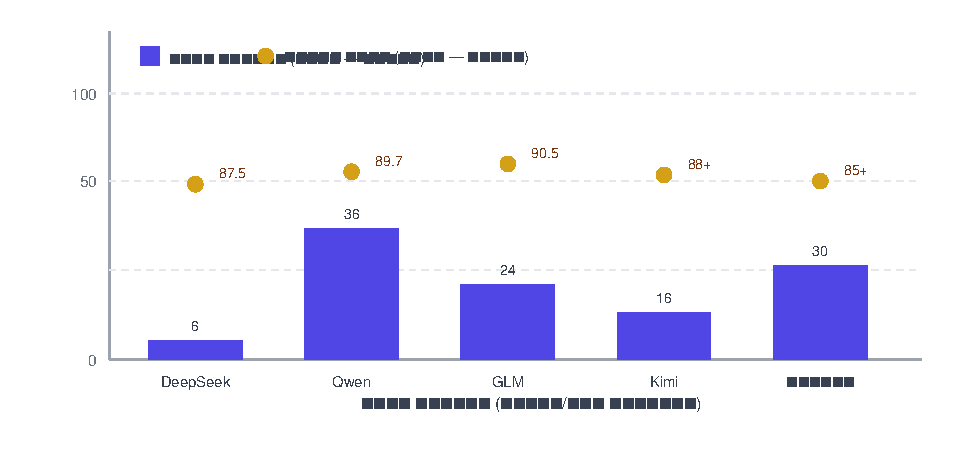
\includegraphics[width=0.92\linewidth]{figures/fig-di-si-shi-er-zhang-1}
\\[2pt]\small Рисунок 4: сравнение пяти моделей по цене и производительности (чем ниже цена и выше балл — тем лучше)
\end{center}

\booksection{Каркас принятия решения при выборе модели}

Узнав особенности моделей, как выбрать модель для своего проекта? Дарим вам «метод четырёх вопросов» — ответьте на четыре вопроса, и вы определите самую подходящую модель.

Проект разворачивается в Китае или за рубежом?

Китай выбирайте китайскую модель

|

Международный доступны зарубежные модели

Основная задача — программирование или что-то другое?

Программирование Claude или DeepSeek

|

Другое продолжаем выбор

Нужен сверхдлинный контекст (>500 тыс. токенов)?

Да Gemini или Kimi

|

Нет продолжаем выбор

Бюджет ограничен?

Да DeepSeek или Qwen-turbo

|

Нет GPT-5.6 или Claude

\begin{center}\small\color{gray}Рисунок 5: метод четырёх вопросов для выбора большой модели\end{center}

\begin{tcbinfo}{Совет: комбинированная стратегия}
Этот метод — не догма: во многих случаях полезно комбинировать несколько моделей. Распространённая стратегия: DeepSeek или Qwen для повседневной разработки (дёшево, хорошо на китайском), Claude для ключевых архитектурных решений (сильные рассуждения, мало галлюцинаций), Gemini для мультимодального анализа (работа с изображениями и видео). Переключайте модели по необходимости, а не «используйте одну до конца».

\end{tcbinfo}

\booksection{Первые шаги с API: подключаем большую модель с нуля}

Многие учебники по AI-программированию учат только работе с чат-интерфейсом, но настоящее «AI-программирование» — когда ваше приложение само вызывает большую модель — идёт через API. API (Application Programming Interface, программный интерфейс приложения) — это протокол общения между программами. Через API ваш код может задействовать возможности большой модели так же просто, как вызывает обычную функцию.

\booksubsection{Что такое токен}

Прежде чем разбираться с API, нужно понять понятие «токен». Токен — базовая единица тарификации больших моделей; её можно назвать «единицей чтения и письма AI». Один токен примерно соответствует 0,75 английского слова (4 символам) или 0,5–1 китайскому иероглифу. Китайский текст в 1000 знаков потребляет примерно 1500–2000 токенов.

Токен — это не количество слов и не количество символов. Большая модель с помощью специального токенизатора (Tokenizer) разбивает текст на токены. Одно и то же слово в разных моделях может занимать разное число токенов: например, «искусственный интеллект» по-китайски — 3 токена в GPT и, возможно, 2 в DeepSeek. API большинства моделей возвращает фактическое число израсходованных токенов — его можно посмотреть в ответе API.

\begin{tcbinfo}{Быстрая оценка стоимости в токенах}
1 миллион китайских знаков — это примерно 1,5 млн токенов. Обработать 1 млн знаков ввода плюс 1 млн знаков вывода с DeepSeek V4 Flash стоит около 0,42 доллара (примерно 3 юаня); с Claude Fable 5 тот же объём — около 60 долларов (примерно 434 юаня). Вот почему выбор модели напрямую влияет на стоимость вашего проекта.

\end{tcbinfo}

\booksubsection{Получение API-ключа}

Первый шаг к работе с API больших моделей — получить API-ключ (API Key), то есть строку-ключ для подтверждения личности. У каждого провайдера моделей своя API-платформа: нужно зарегистрировать аккаунт и создать API-ключ. Ниже — входы на API-платформы основных моделей и порядок получения ключа:

\begin{center}
\begin{tabularx}{\linewidth}{|X|X|X|X|}
\hline
\textbf{Модель} & \textbf{API-платформа} & \textbf{Порядок получения} & \textbf{Бесплатный лимит} \tabularnewline
\hline
DeepSeek & platform.deepseek.com & Регистрация верификация личности создание API-ключа & Бесплатный лимит для новых пользователей \tabularnewline
Tongyi Qianwen & bailian.aliyun.com (платформа Bailian) & Вход с аккаунтом Alibaba Cloud включение сервиса создание ключа & Бесплатный пробный период для новых пользователей \tabularnewline
Zhipu GLM & open.bigmodel.cn & Регистрация верификация личности создание API-ключа & Бесплатный лимит для новых пользователей \tabularnewline
Kimi & platform.moonshot.cn & Регистрация верификация личности создание API-ключа & Ограниченный бесплатный лимит \tabularnewline
Doubao & volcengine.com (Volcano Engine) & Регистрация включение Ark создание API-ключа & Много токенов в подарок за регистрацию \tabularnewline
OpenAI GPT & platform.openai.com & Регистрация привязка кредитной карты создание API-ключа & Без бесплатного лимита (платно) \tabularnewline
Anthropic Claude & console.anthropic.com & Регистрация привязка карты создание API-ключа & Небольшой лимит для новых пользователей \tabularnewline
\hline
\end{tabularx}
\end{center}

\begin{center}\small\color{gray}API-платформы основных моделей и способы получения ключа (август 2026 г.)\end{center}

\textbf{Безопасность: API-ключ = пароль от кошелька}\par

API-ключ равнозначен паролю от вашего кошелька: любой, кто получит ключ, сможет вызывать модели за ваш счёт. Поэтому: никогда не пишите API-ключ прямо в коде (храните его в переменных окружения); никогда не отправляйте код с ключом в публичный Git-репозиторий; никогда не публикуйте в соцсетях скриншоты с ключом. Если ключ утёк, немедленно удалите его на платформе и создайте новый.

\booksubsection{Первый вызов API}

Получив API-ключ, вы можете вызывать API больших моделей на любом языке программирования. Ниже — простейший вызов на Python: отправляем DeepSeek сообщение и получаем ответ.

\begin{lstlisting}[language=Python]
# Установите SDK: pip install openai
# DeepSeek совместим с форматом OpenAI SDK — можно использовать напрямую
from openai import OpenAI
import os

# 1. Создаём клиент (API-ключ читается из переменной окружения)
client = OpenAI(
    api_key=os.environ.get("DEEPSEEK_API_KEY"),
    base_url="https://api.deepseek.com"
)

# 2. Отправляем запрос
response = client.chat.completions.create(
    model="deepseek-chat",  # указываем модель
    messages=[
        {"role": "system", "content": "Ты — ассистент по программированию на Python."},
        {"role": "user", "content": "Напиши функцию быстрой сортировки."}
    ]
)

# 3. Получаем ответ
print(response.choices[0].message.content)

# 4. Смотрим расход токенов
print(f"Входные токены: {response.usage.prompt_tokens}")
print(f"Выходные токены: {response.usage.completion_tokens}")
print(f"Всего токенов: {response.usage.total_tokens}")
\end{lstlisting}

Ключевая логика этого кода: создаём клиент (с API-ключом и адресом модели) формируем список сообщений (system задаёт роль, user — ввод пользователя) отправляем запрос получаем ответ. Этот шаблон подходит почти для всех моделей, совместимых с форматом OpenAI: чтобы сменить модель, достаточно поменять api\_key и base\_url. Именно поэтому многие китайские модели сделали совместимость с форматом OpenAI SDK: разработчику хватает двух строк кода, чтобы переключить модель, — затраты на мигрение минимальны.

Ниже — различия в коде при переключении на другие модели. Обратите внимание: меняются всего две строки:

\begin{lstlisting}[language=Python]
# DeepSeek
client = OpenAI(
    api_key=os.environ.get("DEEPSEEK_API_KEY"),
    base_url="https://api.deepseek.com"
)
# model="deepseek-chat"

# Tongyi Qianwen (платформа Bailian)
client = OpenAI(
    api_key=os.environ.get("DASHSCOPE_API_KEY"),
    base_url="https://dashscope.aliyuncs.com/compatible-mode/v1"
)
# model="qwen-plus"

# Zhipu GLM
client = OpenAI(
    api_key=os.environ.get("GLM_API_KEY"),
    base_url="https://open.bigmodel.cn/api/paas/v4"
)
# model="glm-4"

# OpenAI GPT
client = OpenAI(
    api_key=os.environ.get("OPENAI_API_KEY"),
    # base_url можно оставить по умолчанию
)
# model="gpt-5.6-terra"
\end{lstlisting}

\booksubsection{Потоковые ответы (Streaming)}

В реальных приложениях обычно не хочется ждать, пока AI допишет всё до конца, чтобы показать текст одним куском, — пользователю пришлось бы ждать слишком долго. Потоковый ответ (Streaming) позволяет показывать текст слово за словом по мере генерации, заметно улучшая впечатление от работы. Как на печатной машинке: буквы выпрыгивают одна за другой — ощущения совсем другие.

\begin{lstlisting}[language=Python]
# Потоковый ответ: вывод по символам
stream = client.chat.completions.create(
    model="deepseek-chat",
    messages=[
        {"role": "user", "content": "Напиши туториал по пузырьковой сортировке на Python"}
    ],
    stream=True  # включаем потоковый режим
)

# Получаем по кускам и печатаем
for chunk in stream:
    if chunk.choices[0].delta.content is not None:
        print(chunk.choices[0].delta.content, end="", flush=True)
# Вывод появится посимвольно, как на печатной машинке
\end{lstlisting}

\booksection{Руководство по покупке Token Plan}

У большинства провайдеров моделей два способа тарификации: оплата по мере использования (Pay-as-you-go) и подписочный план (Token Plan / Subscription). Понимание разницы между ними поможет заметно снизить ваши затраты.

\booksubsection{Оплата по использованию или подписка}

\begin{center}
\begin{tabularx}{\linewidth}{|X|X|X|}
\hline
\textbf{Критерий} & \textbf{Оплата по использованию (Pay-as-you-go)} & \textbf{Подписка (Subscription)} \tabularnewline
\hline
Способ оплаты & Платите за фактически израсходованные токены & Фиксированная предоплата за лимит \tabularnewline
Подходит для & Нестабильное потребление, редкие вызовы & Стабильное потребление, частые вызовы \tabularnewline
Ценовое преимущество & Стандартная цена & На 20–50\% ниже оплаты по использованию \tabularnewline
Гибкость & Доступно в любой момент, без обязательств & Нужна предоплата; лимит может сгореть \tabularnewline
Превышение лимита & Автоматический переход к оплате по использованию & После исчерпания лимита — оплата по использованию \tabularnewline
Типичные платформы & Официальные API-платформы каждой модели & OpenAI Plus/Pro, Claude Pro, Cursor Pro \tabularnewline
\hline
\end{tabularx}
\end{center}

\begin{center}\small\color{gray}Сравнение двух способов оплаты\end{center}

Новичкам советуем начинать с оплаты по использованию: без предоплаты, платите ровно за то, что потратили. Когда месячное потребление стабилизируется (например, превысит 50 юаней в месяц), подумайте о переходе на подписку ради более низкой цены за единицу.

\booksubsection{Обзор популярных подписок}

\begin{center}
\begin{tabularx}{\linewidth}{|X|X|X|X|}
\hline
\textbf{План} & \textbf{Цена в месяц} & \textbf{Что входит} & \textbf{Кому подходит} \tabularnewline
\hline
ChatGPT Free & Бесплатно & Безлимитный текстовый чат с GPT-5.6 Luna & Проба для новичков с нуля \tabularnewline
ChatGPT Plus & 20 долл./мес & GPT-5.6 Sol, генерация изображений, анализ данных, доступ к плагинам & Умеренно активные пользователи \tabularnewline
ChatGPT Pro & 200 долл./мес & Безлимитный доступ ко всем моделям, приоритетный доступ к новинкам & Профессионалы с высокой нагрузкой \tabularnewline
Claude Free & Бесплатно & Ограниченное число диалогов с Claude & Проба для новичков с нуля \tabularnewline
Claude Pro & 20 долл./мес & Безлимитное использование Claude, приоритетный доступ к новым моделям & Разработчики \tabularnewline
Cursor Free & Бесплатно & Ограниченное число AI-дополнений и диалогов & Проба для начинающих \tabularnewline
Cursor Pro & 20 долл./мес & Безлимитные AI-дополнения, 500 премиум-запросов в месяц & Разработчики на каждый день \tabularnewline
Cursor Business & 40 долл./мес за человека & Командная работа, панель администратора, режим приватности & Команды \tabularnewline
\hline
\end{tabularx}
\end{center}

\begin{center}\small\color{gray}Подписки популярных AI-инструментов (август 2026 г.)\end{center}

У китайских моделей подписочные схемы немного другие. DeepSeek работает в основном по оплате за использование — месячных подписок нет: вы пополняете счёт и платите по факту. Tongyi Qianwen на платформе Bailian предлагает предоплаченные пакеты ресурсов (покупаете определённый объём токенов со скидкой). У Doubao на Volcano Engine есть похожие предоплаченные схемы. Для китайских разработчиков самая экономная комбинация обычно такая: DeepSeek с оплатой по использованию (повседневная разработка) + бесплатные лимиты Doubao (пробы и тесты).

\booksubsection{Платформы-агрегаторы API}

Если нужно пользоваться сразу несколькими моделями, платформа-агрегатор API — беспроблемный выбор. Агрегатор даёт один общий API-ключ, с которым доступны десятки моделей по всему миру, — регистрироваться отдельно на каждой платформе не придётся.

\begin{center}
\begin{tabularx}{\linewidth}{|X|X|X|X|}
\hline
\textbf{Платформа} & \textbf{Особенности} & \textbf{Ценовое преимущество} & \textbf{Подходит для} \tabularnewline
\hline
OpenRouter (openrouter.ai) & Международный агрегатор: один ключ открывает модели всего мира & Прозрачные цены, сравнение в реальном времени & Тем, кто гибко переключается между зарубежными моделями \tabularnewline
SiliconFlow (siliconflow.cn) & Китайский агрегатор: API множества китайских моделей & На 20–30\% ниже официальных цен & Китайские разработчики, сравнение цен между моделями \tabularnewline
Azure OpenAI (прокси Microsoft) & API OpenAI через прокси Microsoft Azure & Batch API даёт скидку 50\% & Корпоративные вызовы OpenAI, крупные асинхронные задачи \tabularnewline
Baidu Qianfan (qianfan.baidubce.com) & Облачная AI-платформа Baidu: модели ERNIE (Wenxin) и другие & Бесплатный лимит для новых пользователей & Пользователи экосистемы Baidu \tabularnewline
\hline
\end{tabularx}
\end{center}

\begin{center}\small\color{gray}Популярные агрегаторы API (август 2026 г.)\end{center}

\textbf{Осторожно: не покупайте «общие ключи»}\par

Не покупайте так называемые «общие API-ключи» на Taobao, Xianyu и подобных площадках: происхождение таких ключей неизвестно, аккаунт могут заблокировать в любой момент, плюс есть риск утечки данных. Получайте API-ключи только через официальные или проверенные платформы-агрегаторы.

\booksubsection{Стратегии экономии}

Правильно выбранная модель — только первый шаг; не менее важно «пользоваться экономно». Вот несколько проверенных на практике стратегий снижения затрат:

\begin{enumerate}
  \item Используйте попадания в кэш. У многих моделей есть «кэширование»: если в запросе есть уже обработанное ранее содержимое (например, системный промпт), эта часть тарифицируется по очень низкой цене. У DeepSeek попадание в кэш стоит всего 1/60 обычной цены. Ставьте фиксированный системный промпт в начало списка сообщений — так вы максимизируете попадания в кэш.
  \item Многоуровневая маршрутизация: простые задачи — дешёвой модели, сложные — дорогой. Например, DeepSeek V4 Flash для классификации текстов (вывод 2 юаня за миллион токенов), а Claude — для архитектурного проектирования (вывод 181 юань за миллион токенов). В проекте около 80\% вызовов можно отдать дешёвой модели.
  \item Ограничивайте длину вывода. API тарифицируется по токенам вывода: чем длиннее вывод, тем дороже. Если пространные рассуждения не нужны, задайте параметр max\_tokens, чтобы ограничить длину ответа и не дать AI «лить воду».
  \item Используйте Batch API для задач без реального времени. Если у вас много задач, не требующих мгновенного ответа (массовая разметка данных, сводки документов и т. п.), Batch API даёт скидку 50\%. Эту функцию предлагают и OpenAI, и Azure.
  \item Следите за расходом токенов. Большинство API-платформ предлагают панели статистики. Регулярно смотрите распределение расходов, находите самые «токенозатратные» вызовы и точечно их оптимизируйте. Маленькая правка промпта (например, заменить «объясните подробно» на «объясните в трёх предложениях») может сэкономить до 50\% токенов.
\end{enumerate}

\begin{center}
\begin{tabularx}{\linewidth}{|X|X|X|X|}
\hline
\textbf{Стратегия оптимизации} & \textbf{Экономия} & \textbf{Сложность внедрения} & \textbf{Пояснение} \tabularnewline
\hline
Попадания в кэш & До 98\% & Низкая & Фиксированное содержимое — в начало сообщений \tabularnewline
Многоуровневая маршрутизация & 50\%-80\% & Средняя & Простые задачи — дешёвой модели \tabularnewline
Ограничение длины вывода & 30\%-60\% & Низкая & Задайте параметр max\_tokens \tabularnewline
Batch API & 50\% & Низкая & Пакетная обработка отложенных задач \tabularnewline
Оптимизация промптов & 20\%-50\% & Средняя & Сокращайте промпты, убирайте избыточность \tabularnewline
\hline
\end{tabularx}
\end{center}

\begin{center}\small\color{gray}Стратегии экономии и их эффект (август 2026 г.)\end{center}

\booksection{Практика: подключаем API большой модели в проекте}

Завершим главу полноценной практикой — создадим «генератор резюме на AI»: пользователь вводит длинный текст, а мы вызываем API большой модели и получаем выжимку. Эта практика покажет полный цикл работы с API: настройку окружения, вызов API, обработку ошибок и контроль затрат.

\begin{lstlisting}[language=Python]
# ai_summarizer.py - ИИ-суммаризатор
import os
from openai import OpenAI

# 1. Настройка (API-ключ читается из переменной окружения — никогда не вшивайте его в код)
client = OpenAI(
    api_key=os.environ.get("DEEPSEEK_API_KEY"),
    base_url="https://api.deepseek.com"
)

def summarize(text: str, max_length: int = 200) -> dict:
    """Суммаризация текста

    Args:
        text: исходный текст для суммаризации
        max_length: максимальная длина резюме (в токенах)

    Returns:
        dict: резюме и сведения о расходе токенов
    """
    try:
        response = client.chat.completions.create(
            model="deepseek-chat",
            messages=[
                {
                    "role": "system",
                    "content": "Ты — генератор резюме."
                               "Кратко резюмируй предоставленный пользователем текст."
                               "Резюме — не длиннее 3 предложений."
                },
                {
                    "role": "user",
                    "content": f"Суммаризируй следующий текст:\n\n{text}"
                }
            ],
            max_tokens=max_length,  # ограничиваем длину вывода
            temperature=0.3  # низкая температура = стабильнее
        )

        return {
            "success": True,
            "summary": response.choices[0].message.content,
            "input_tokens": response.usage.prompt_tokens,
            "output_tokens": response.usage.completion_tokens,
            "total_tokens": response.usage.total_tokens
        }

    except Exception as e:
        return {
            "success": False,
            "error": str(e)
        }

# 2. Пример использования
if __name__ == "__main__":
    long_text = """
    (вставьте сюда длинный текст…)
    """

    result = summarize(long_text)

    if result["success"]:
        print(f"Резюме: {result['summary']}")
        print(f"Потрачено токенов: {result['total_tokens']}")
        # оцениваем стоимость: DeepSeek V4 Flash
        cost = result['total_tokens'] * 0.000004  # $\approx$0,4 фэня за 1 000 токенов
        print(f"Ожидаемая стоимость: {cost:.4f} юаня")
    else:
        print(f"Ошибка: {result['error']}")
\end{lstlisting}

Этот код воплощает несколько лучших практик работы с API: API-ключ читается из переменных окружения и никогда не зашивается в код; у функции понятная документация и подсказки типов; параметр max\_tokens ограничивает длину вывода; temperature задан низким (0.3) для более стабильного вывода; есть полноценная обработка ошибок; возвращается информация о расходе токенов для контроля затрат. Когда поручите этот код AI, просто перечислите ему эти требования — он вполне способен их реализовать.

Главный итог главы: модели — это «боеприпасы», методология — «тактика». Правильные боеприпасы облегчают бой, но без хорошей тактики даже лучшие патроны войну не выиграют. Теперь вы знаете особенности моделей и умеете работать с API — ваш «арсенал» полон, но как вести этот бой, решают методы мышления из предыдущих глав.

\begin{tcbpractice}{Попробуйте сами: добейтесь первого успешного вызова API}
Зарегистрируйтесь на платформе китайской модели (рекомендуем DeepSeek или Zhipu — оба дарят лимиты новым пользователям), создайте API-ключ, запишите его в переменные окружения системы (не в код!), затем запустите код из раздела «Первый вызов API». В тот момент, когда вы увидите напечатанный ответ AI, вы перейдёте границу между «пользоваться AI» и «создавать AI-приложения».

\end{tcbpractice}

\begin{tcbsummary}{Итоги главы}
\begin{itemize}
  \item Международная тройка лидеров: GPT-5.6 (сбалансированный универсал), Claude (эталон программирования + всего 1\% галлюцинаций), Gemini (король мультимодальности + контекст 2 млн)
  \item Китайская пятёрка: DeepSeek V4 (король цены и качества; следите за анонсом повышения цен), Qwen3.7 (корпоративный уровень), GLM-5.1 (№1 в SWE среди китайских моделей), Kimi K3 (сверхдлинные тексты), Doubao (бесплатный старт)
  \item Метод четырёх вопросов: где развёртывание? программирование или другое? нужен сверхдлинный контекст? важен бюджет?
  \item Токен — единица тарификации: 1 китайский знак — примерно 1,5–2 токена; 1 млн знаков — примерно 1,5 млн токенов
  \item API-ключ = пароль от кошелька: храните в переменных окружения, никогда не зашивайте в код и не отправляйте в Git
  \item Китайские модели обычно совместимы с OpenAI SDK: для смены модели достаточно поменять две строки — api\_key и base\_url
  \item Пять приёмов экономии: попадания в кэш, многоуровневая маршрутизация, ограничение вывода, Batch API, контроль расхода
\end{itemize}

\end{tcbsummary}
